%\section{GUI - Package Structure}
%\begin{figure}[!ht]
%\begin{center}
%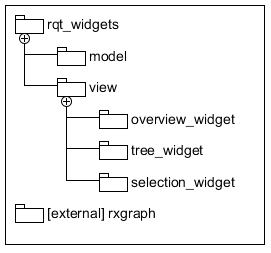
\includegraphics[scale=1.0]{./bilder/package_structure_gui.png}
%\caption{The package structure of the GUI}
%\label{The package structure of the GUI}
%\end{center}
%\end{figure}

%\mbox{}

%\newpage
\section{GUI}
\begin{figure}[!ht]
\begin{center}
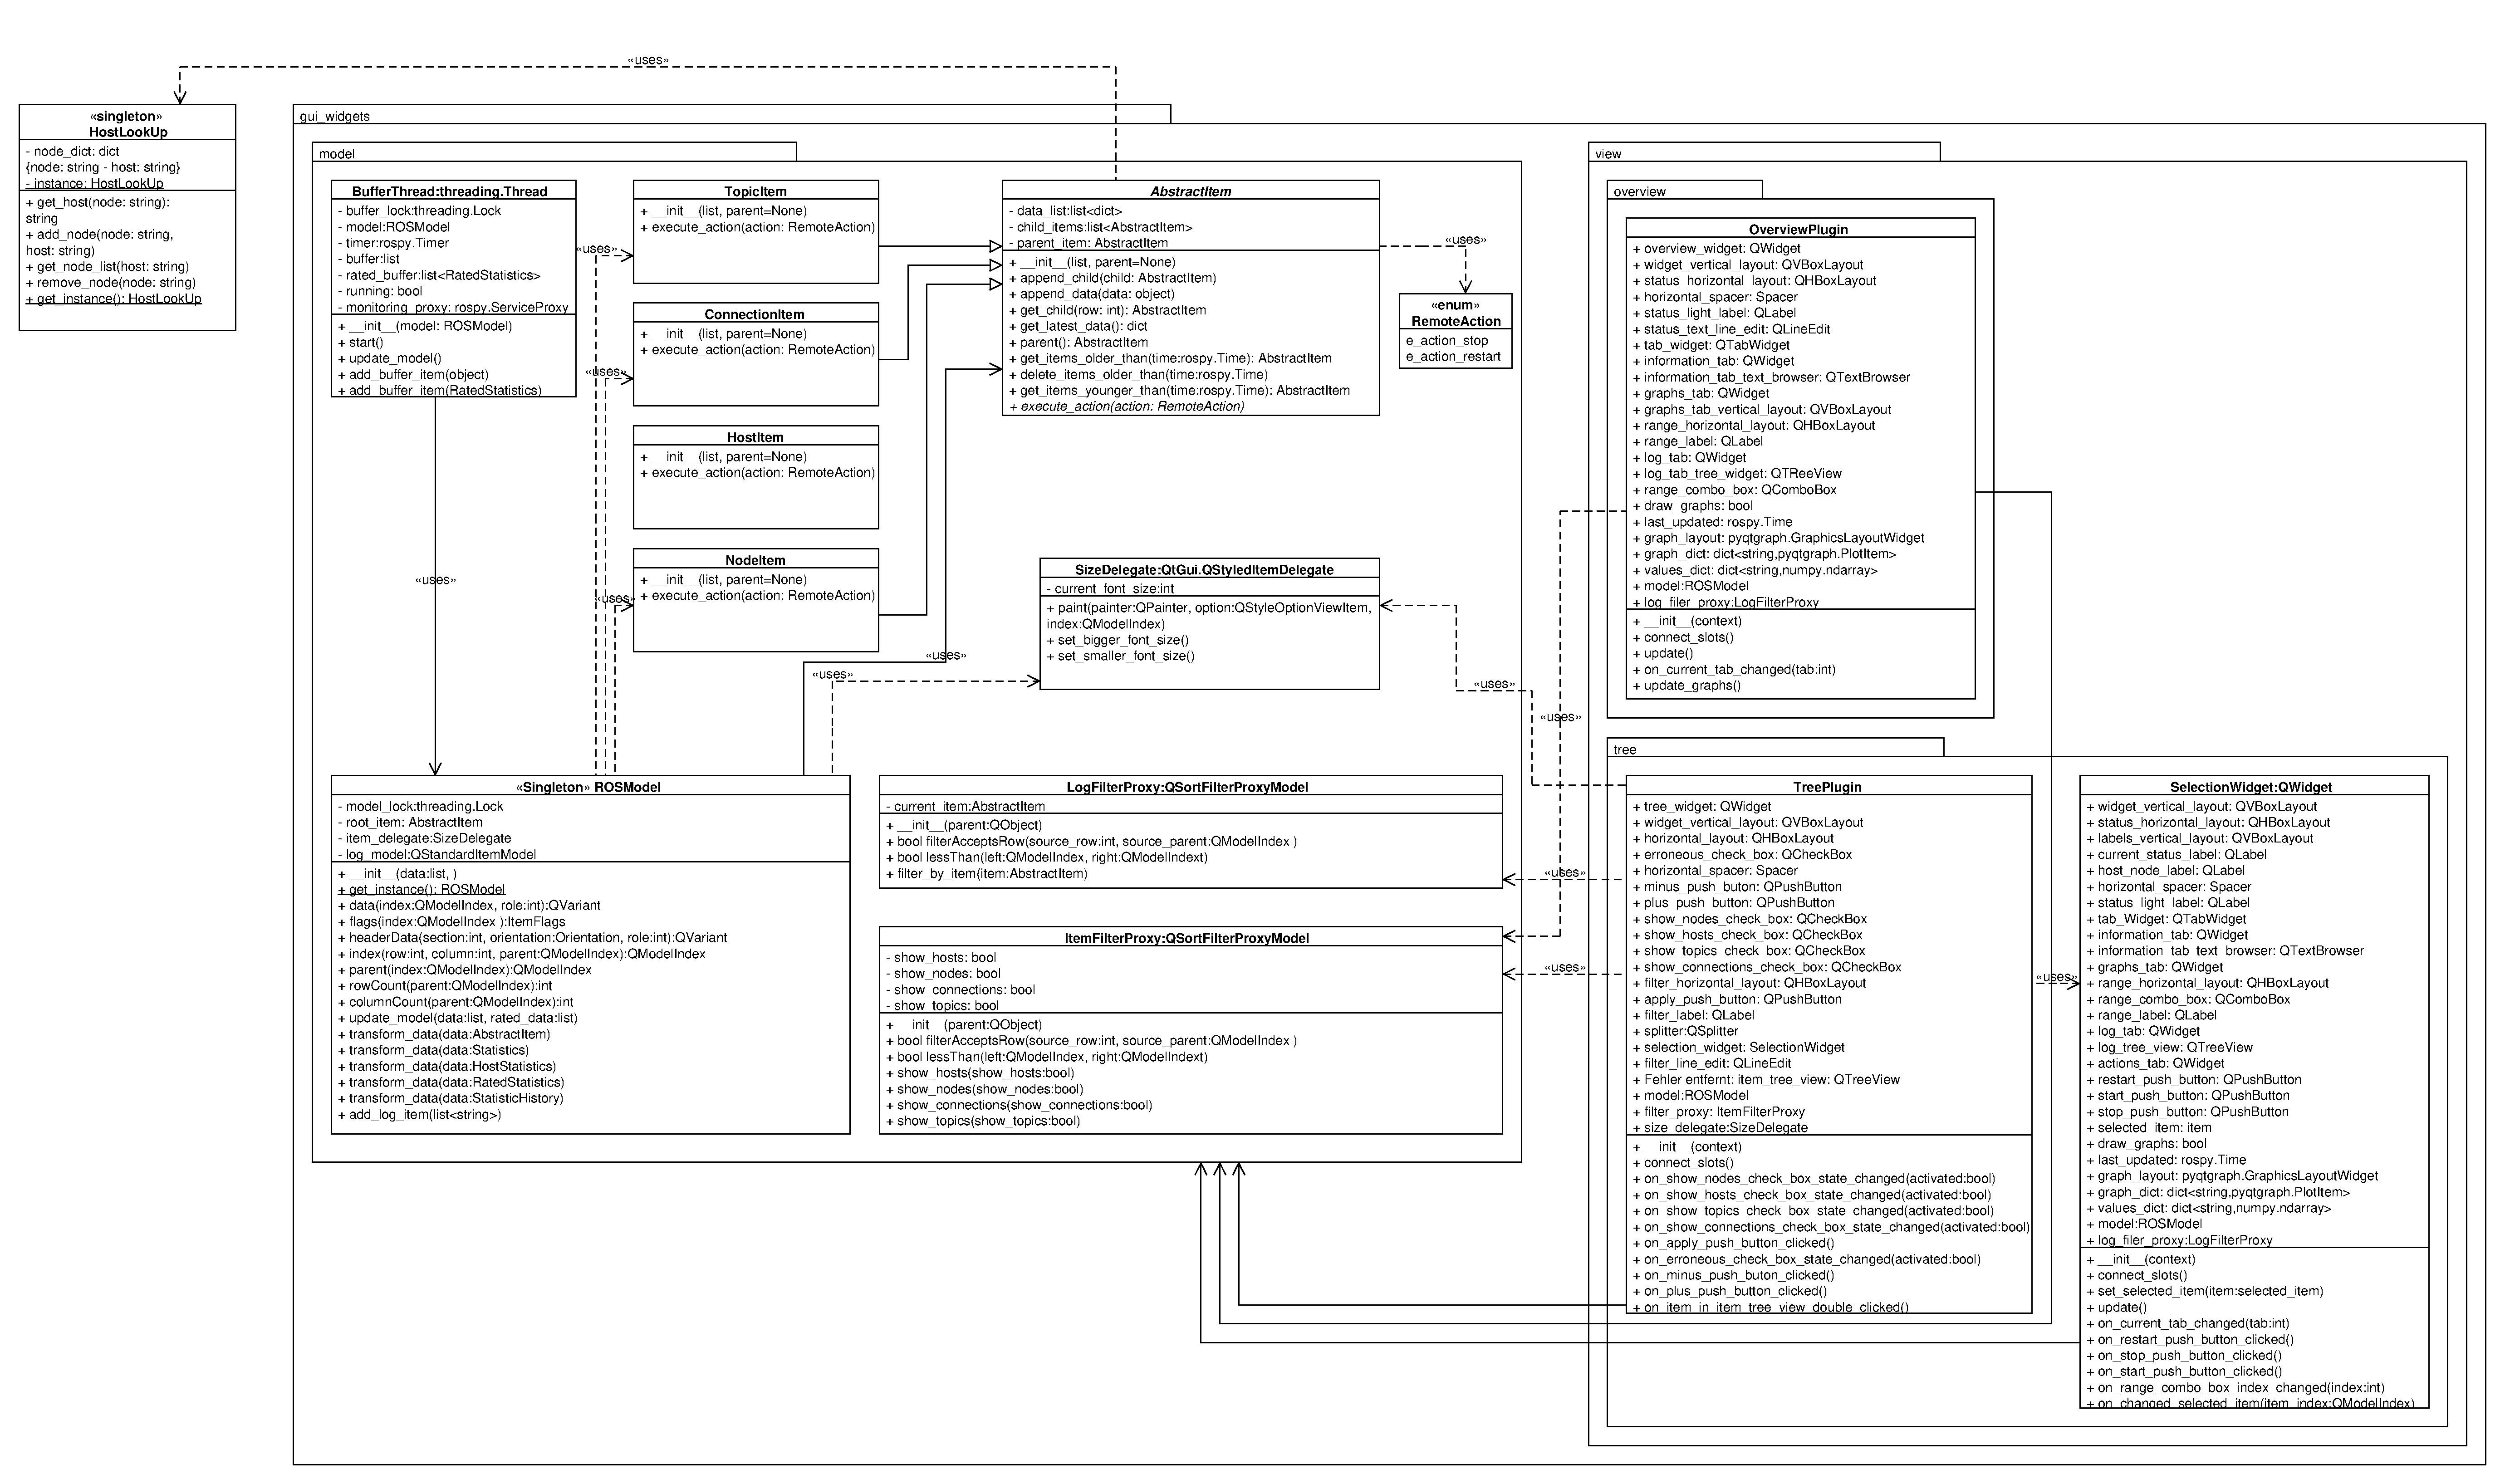
\includegraphics[width=1.0\linewidth]{./diagram_pictures/KlassendiagrammWidgets.pdf}
\caption{The GUI class diagram}
\end{center}
\end{figure}

\newpage
\section{GUI - Model}
\begin{figure}[!ht]
\begin{center}
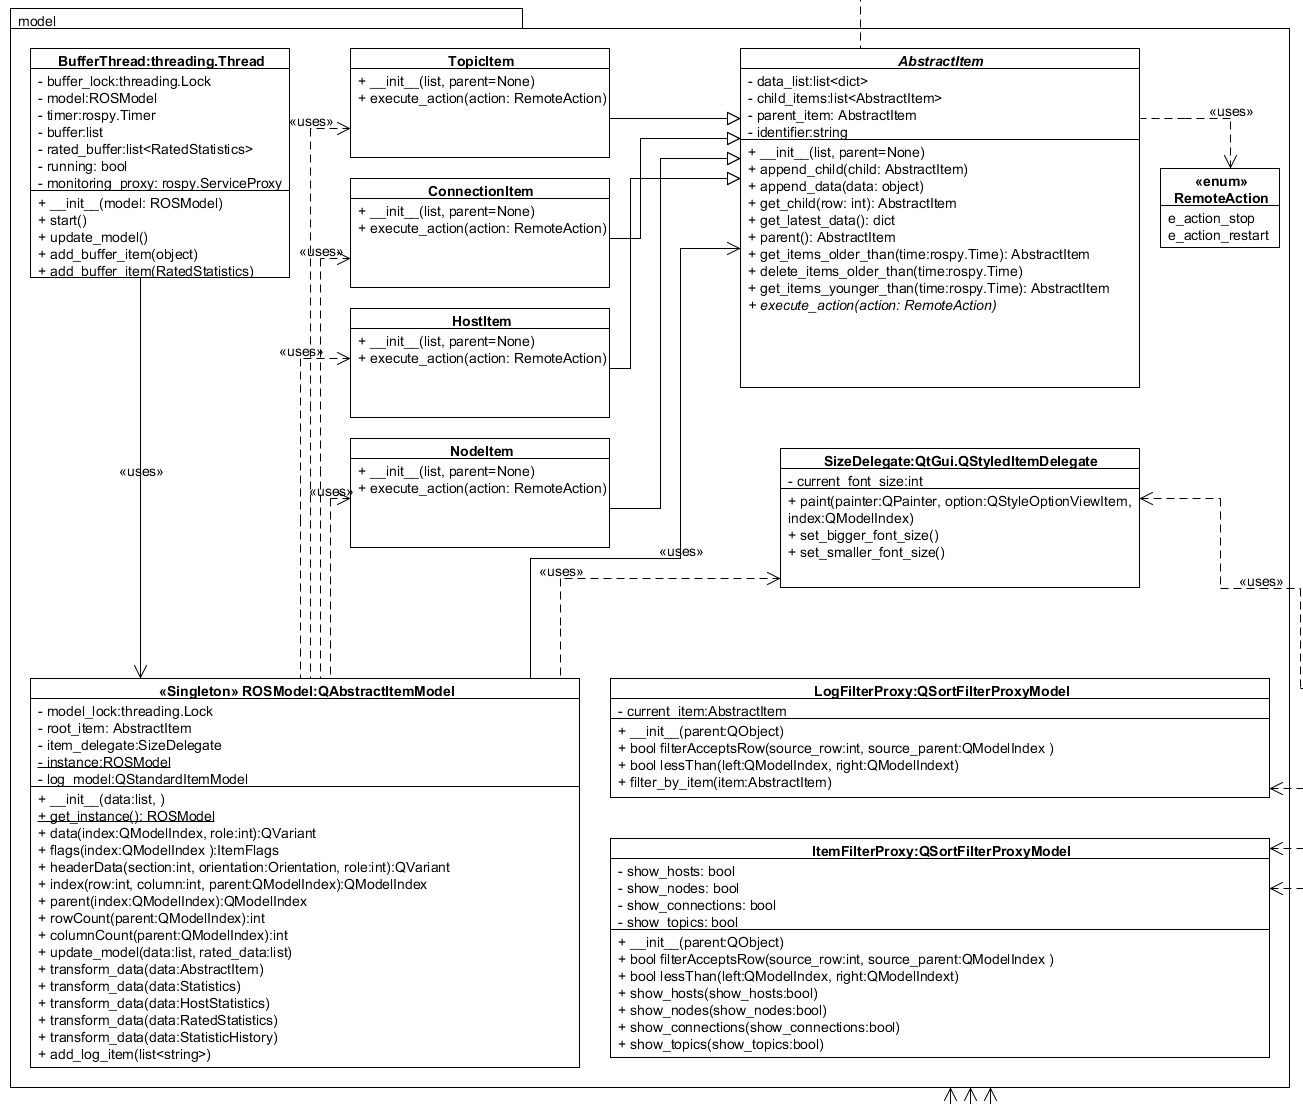
\includegraphics[width=1.0\linewidth]{./diagram_pictures/model.png}
\caption{The model class diagram}
\end{center}
\end{figure}

\newpage
\subsection{BufferThread}
\begin{figure}[htbp]
	\begin{minipage}[t]{7cm}
		\vspace{0pt}
		\centering
		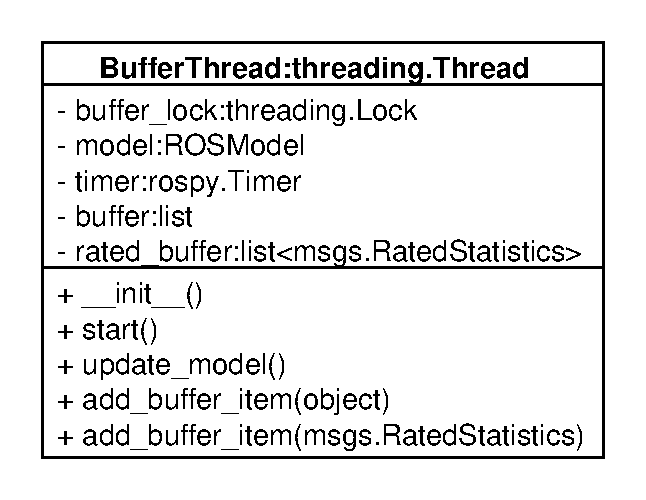
\includegraphics[scale=0.6]{./diagram_pictures/BufferThread.pdf}
		\caption{The BufferThread}
	\end{minipage}
	\hfill
	\begin{minipage}[t]{8cm}
		\vspace{10pt}
		This thread should buffer the incoming data from the topics and regulary
		update the model.
	\end{minipage}
\end{figure}
\subsubsection{Attributes}
\begin{itemize}
  \item \textbf{private threading.Lock buffer\_lock} \\
  The lock that guards the buffer from getting modified parallely
  \item \textbf{private ROSModel model}\\ 
  The model of the hosts/nodes/topics/connections
  \item \textbf{private rospy.Timer timer} \\
  ROS Timer which regularily calls update\_model()
  \item \textbf{private list buffer}\\
  Buffers the tons of incomming data by
  simply storing it here together with a timestamp for later usage
%   \item \textbf{private okcdob\_oqq:rospy.OkcdobOqq}\\ 
%   Drsc sc kx okcdob oqq. Myxqbkdevkdsyxc.
  \item \textbf{private list<RatedStatistics> rated\_buffer}\\ 
  A list for the incoming RatedStatistics items, stored here for later
  processing.
  \item \textbf{private bool running}\\
  Is true if the thread is running
  \item \textbf{private rospy.ServiceProxy monitoring\_proxy}\\ 
  The proxy to the monitoring node for obtaining statistics and rated
  statistics of the past minutes. To be called only once when the GUI started
  and the MonitoringNode has been running for a while
\end{itemize}
\subsubsection{Methods}
\begin{itemize}
%  \item \textbf{public \_\_init\_\_()} 
  \item \textbf{public void start()}\\
  Starts the thread and also the timer for regulary updates of the model. It is ensured via the running attribute that this function cannot be called multiple times.
  \item \textbf{public void update\_model()}\\ 
  Starts the update of the model. Will be called regulary by the timer. Will first read the data from the buffer and add the according data items to the items of the model and afterwards use the rated\_buffer to add a rating to these entries.
  \item \textbf{public void add\_buffer\_item(object message)}\\ 
  Adds the item to the buffer list. Will be called whenever data from the topics
  is available.
  \item \textbf{public void add\_buffer\_item(RatedStatistics message)}\\
  Adds the RatedStatistics item to the rated\_buffer
\end{itemize}

\subsection{ROSModel}
\begin{figure}[htbp]
	\begin{minipage}[t]{7cm}
		\vspace{0pt}
		\centering
		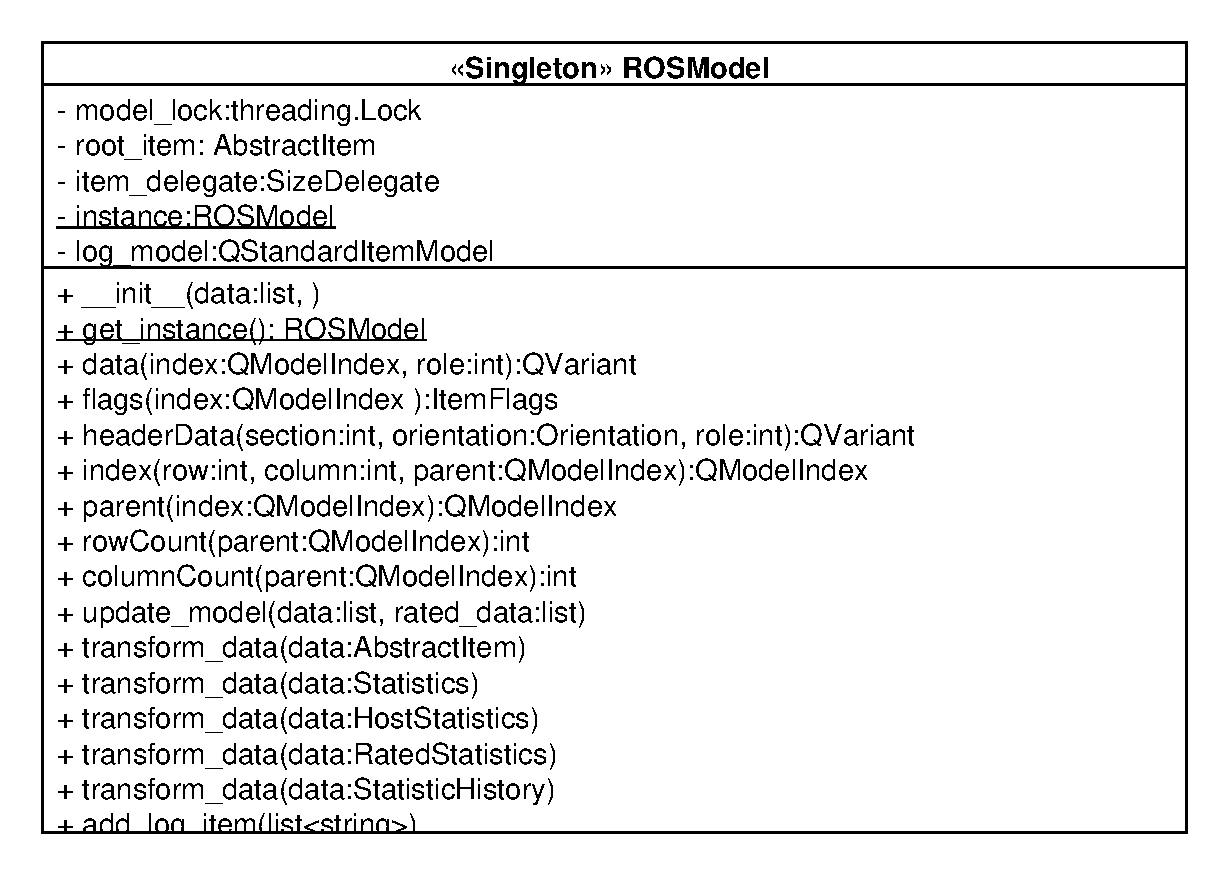
\includegraphics[scale=0.6]{./diagram_pictures/ROSModel.pdf}
		\caption{The ROSModel}
	\end{minipage}
	\hfill
	\begin{minipage}[t]{6cm}
		\vspace{10pt}		
		Represents the data as a QtModel. This enables automated updates of the View.
	\end{minipage}
\end{figure}
\subsubsection{Attributes}
\begin{itemize}
 % \item \textbf{private item\_list: list}
  \item \textbf{private threading.Lock model\_lock}\\ 
  Protects the model from parallel modification
  \item \textbf{private AbstractItem root\_item}\\
  Contains the list of headers
  \item \textbf{private SizeDelegate item\_delegate}\\
  The item\_delegate is responsible for painting the rows in a specific manner e.g. to make the font bigger.
  \item \textbf{private QStandardItemModel log\_model}\\ The model which is used for representing the log data
  \item \textbf{private static ROSModel instance}\\
   The static instance for the Singleton
   
\end{itemize}
\subsubsection{Methods}
\begin{itemize}
  \item \textbf{public \_\_init\_\_()}\\ 
  Defines the class attributes especially the root\_item which later contains the list of headers e.g. for a TreeView representation
  \item \textbf{public ROSModel get\_instance()}\\
  Returns the instance of the ROSModel
  \item \textbf{public QVariant data(QModelIndex index, int role)}\\
  Returns the data of an item at the given index
  \item \textbf{public ItemFlags flags(QModelIndex index)}\\
  Returns the flags of the item at the given index (like Qt::ItemIsEnabled)
  \item \textbf{public QVariant headerData(int section, Orientation orientation, int role)}\\ 
  Returns the headerData  at the given section
  \item \textbf{public QModelIndex index(int row, int column, QModelIndex parent)}\\
  Returns the index of an item at the given column/row
  \item \textbf{public QModelIndex parent(QModelIndex index)}\\ 
  Returns the QModelIndex of the parent of the child item specified via its index
  \item \textbf{public int rowCount(QModelIndex index)}\\ 
  Returns the amount of rows in the model
  \item \textbf{public int columnCount(QModelIndex index)}\\
  Returns the amount of columns in the model
  \item \textbf{public void update\_model(list data, list ratd\_data)}\\ 
  Updates the model by using the items of the list. The items will be of the message types 
  \item \textbf{public void transform\_data(Statistics data)}\\ 
  Integrates a TopicStatistics in the model by modifing its item/s by adding a new dict to the corresponding item (especially the TopicItem and the ConnectionItem)
  \item \textbf{public void transform\_data(NodeStatistics data)}\\ 
  Integrates a NodeStatistics in the model by modifing its item/s by adding a new dict with the entries of the given parameter
  \item \textbf{public void transform\_data(HostStatistics data)}\\ 
  Integrates a HostStatistics in the model by modifing its item/s by adding a new dict with the entries of the given parameter
  \item \textbf{public void transform\_data(RatedStatistics data)}\\ 
  Add the rating to an existing entry by modifing the dict of the corresponding
  item/s
  \item \textbf{public void transform\_data(StatisticHistory data)}\\ 
  When using the monitor\_proxy to receive about the last minutes from the monitoring node
  it returns a StaticHistory item which can then be integrated in the model via this method
  \item\textbf{public void add\_log\_item(list<string>)}\\
  Adds the given list as a log entry to the model
  \end{itemize}

\subsection{AbstractItem}
\begin{figure}[htbp]
	\begin{minipage}[t]{7cm}
		\vspace{0pt}
		\centering
		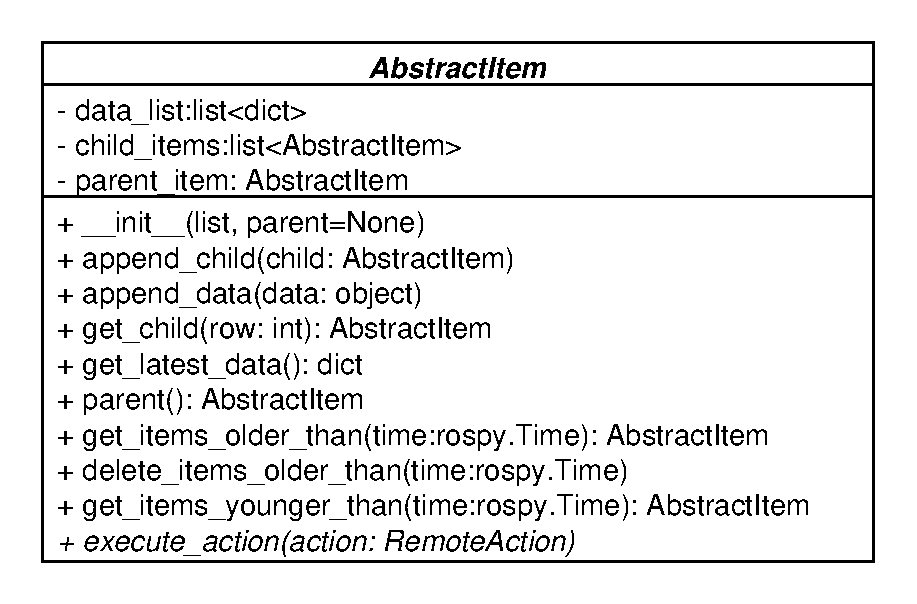
\includegraphics[scale=0.6]{./diagram_pictures/AbstractItem.pdf}
		\caption{The AbstractItem}
	\end{minipage}
	\hfill
	\begin{minipage}[t]{6cm}
		\vspace{10pt}		
		Provides a unified interface to access the items of a model.
	\end{minipage}
\end{figure}
\subsubsection{Attributes}
\begin{itemize}
  \item \textbf{private list<dict> data\_list}\\ 
  Contains the data of the abstract item including a time stamp so that
  the progress in time can be shown
  \item \textbf{private list<AbstractItem> child\_items}\\ 
  The childs of this item
  \item \textbf{private AbstractItem parent\_item}\\ 
  The parent of this item
\end{itemize}
\subsubsection{Methods}
\begin{itemize}
%  \item \textbf{public \_\_init(list, parent=None)\_\_}
   \item \textbf{public void append\_child(AbstractItem child)}\\ 
   Append a child to the list of childs
  \item \textbf{public void append\_data(oject data)}\\ 
  Append data to the data\_list of the AbstractItem
  \item \textbf{public AbstractItem get\_child(int row)}\\ 
  Returns the child at the position row
  \item \textbf{public dict get\_latest\_data()}\\ 
  Returns the latest dict of the data\_list 
  \item \textbf{public AbstractItem parent()}\\ 
  Returns the parent of this or None if there is none
  \item \textbf{public AbstractItem get\_items\_older\_than(rospy.Time time)}\\
  Returns all items wich are older than \textit{rospy.Time}
  \item \textbf{public void delete\_items\_older\_than(rospy.Time time})\\
  Deletes all items wich are older than \textit{rospy.Time}
  \item \textbf{public AbstractItem get\_items\_younger\_than(rospy.Time)}\\
  Returns all items wich are younger than \textit{rospy.Time time}
  \item \textbf{public abstract void execute\_action(RemoteAction action)}\\ 
  Executes a action on the current item like stop or restart. Calls to this
  method should be redirected to the remote host on executed there.
\end{itemize}

\newpage
\subsection{HostItem}
\begin{figure}[htbp]
	\begin{minipage}[t]{7cm}
		\vspace{0pt}
		\centering
		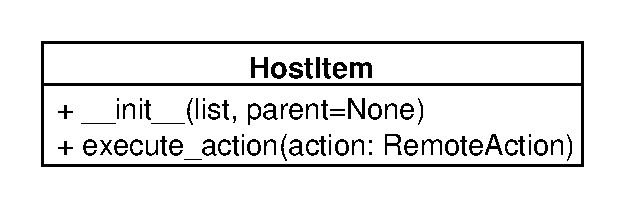
\includegraphics[scale=0.6]{./diagram_pictures/HostItem.pdf}
		\caption{The HostItem}
	\end{minipage}
	\hfill
	\begin{minipage}[t]{8cm}
		\vspace{10pt}		
		A HostItem represents a host with all its data.
	\end{minipage}
\end{figure}
\subsubsection{Methods}
\begin{itemize}
%  \item \textbf{public \_\_init(list, parent=None)\_\_}
  \item \textbf{public execute\_action(RemoteAction action)}\\
  Sends a signal to stop or restart a node
\end{itemize}

\subsection{NodeItem}
\begin{figure}[htbp]
	\begin{minipage}[t]{7cm}
		\vspace{0pt}
		\centering
		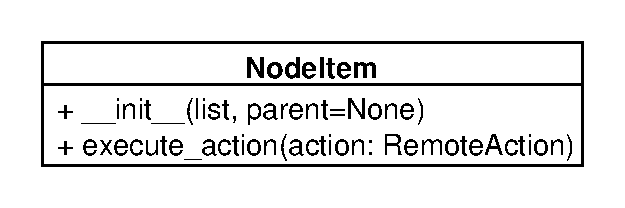
\includegraphics[scale=0.6]{./diagram_pictures/NodeItem.pdf}
		\caption{The NodeItem}
	\end{minipage}
	\hfill
	\begin{minipage}[t]{8cm}
		\vspace{10pt}		
		A NodeItem represents a node with all of its data. It also has a interface to
		start/stop/restart nodes.
	\end{minipage}
\end{figure} 
\subsubsection{Methods}
\begin{itemize}
 % \item \textbf{public \_\_init(list, parent=None)\_\_}
  \item \textbf{public execute\_action(RemoteAction action)}\\
  Sends a signal to stop or restart the node
\end{itemize}

\subsection{TopicItem}
\begin{figure}[htbp]
	\begin{minipage}[t]{7cm}
		\vspace{0pt}
		\centering
		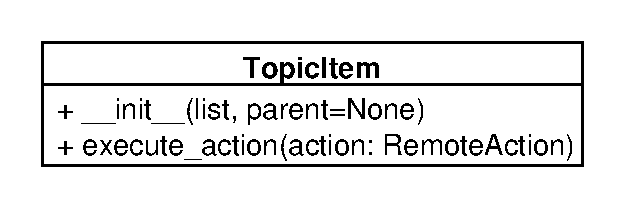
\includegraphics[scale=0.6]{./diagram_pictures/TopicItem.pdf}
		\caption{The TopicItem}
	\end{minipage}
	\hfill
	\begin{minipage}[t]{8cm}
		\vspace{10pt}		
		A TopicItem reprensents a specific topic which contains many connections and has attributes like the number of sent messages.
	\end{minipage}
\end{figure} 
\subsubsection{Methods}
\begin{itemize}
%  \item \textbf{public \_\_init(list, parent=None)\_\_}
  \item \textbf{public execute\_action(RemoteAction action)}\\ 
  Not senseful, throws an exception
\end{itemize}

\subsection{ConnectionItem}
\begin{figure}[htbp]
	\begin{minipage}[t]{7cm}
		\vspace{0pt}
		\centering
		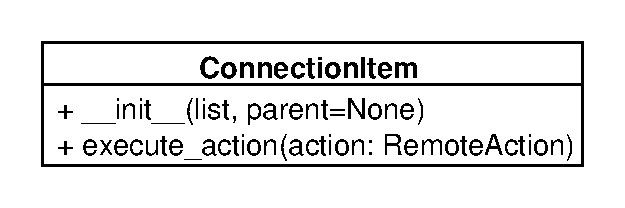
\includegraphics[scale=0.6]{./diagram_pictures/ConnectionItem.pdf}
		\caption{The ConnectionItem}
	\end{minipage}
	\hfill
	\begin{minipage}[t]{8cm}
		\vspace{10pt}
		A ConnectionItem reprensents the connection between a publisher and a
		subscriber and the topic they are puglishing / listenening on.
	\end{minipage}
\end{figure}  
\subsubsection{Methods}
\begin{itemize}
%  \item \textbf{public \_\_init(list, parent=None)\_\_}
  \item \textbf{public execute\_action(RemoteAction action)}\\ 
  Not senseful, throws an exception
\end{itemize}

% \subsection{TimeStampedData}
% ..
% \subsubsection{Attributes}
% \begin{itemize}
%   \item \textbf{private data: object}
%   ..
%   \item \textbf{private time\_stamp: datetime.time}
%   ..
% \end{itemize}
% \subsubsection{Methods}
% \begin{itemize}
%   \item \textbf{public \_\_init(object, datetime.time)\_\_}
%   ..
%   \item \textbf{public datetime.time get\_time\_stamp()}
%   ..
%   \item \textbf{public object get\_data()}
%   ..
% \end{itemize}

\subsection{Enum RemoteAction}
\begin{figure}[htbp]
	\begin{minipage}[t]{7cm}
		\vspace{0pt}
		\centering
		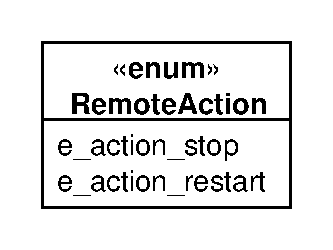
\includegraphics[scale=0.6]{./diagram_pictures/RemoteAction.pdf}
		\caption{The ROSModel}
	\end{minipage}
	\hfill
	\begin{minipage}[t]{8cm}
		\vspace{10pt}
		Gives a predefinition for a remote interaction with hosts and nodes.
	\end{minipage}
\end{figure}  
\subsubsection{Types}
\begin{itemize}
	\item \textbf{e\_action\_stop}\\
	The action that should stop a host or node
	\item \textbf{e\_action\_restart}\\
	The action that should restart a host or node
\end{itemize}

\newpage
\subsection{ItemFilterProxy}
\begin{figure}[htbp]
	\begin{minipage}[t]{7cm}
		\vspace{0pt}
		\centering
		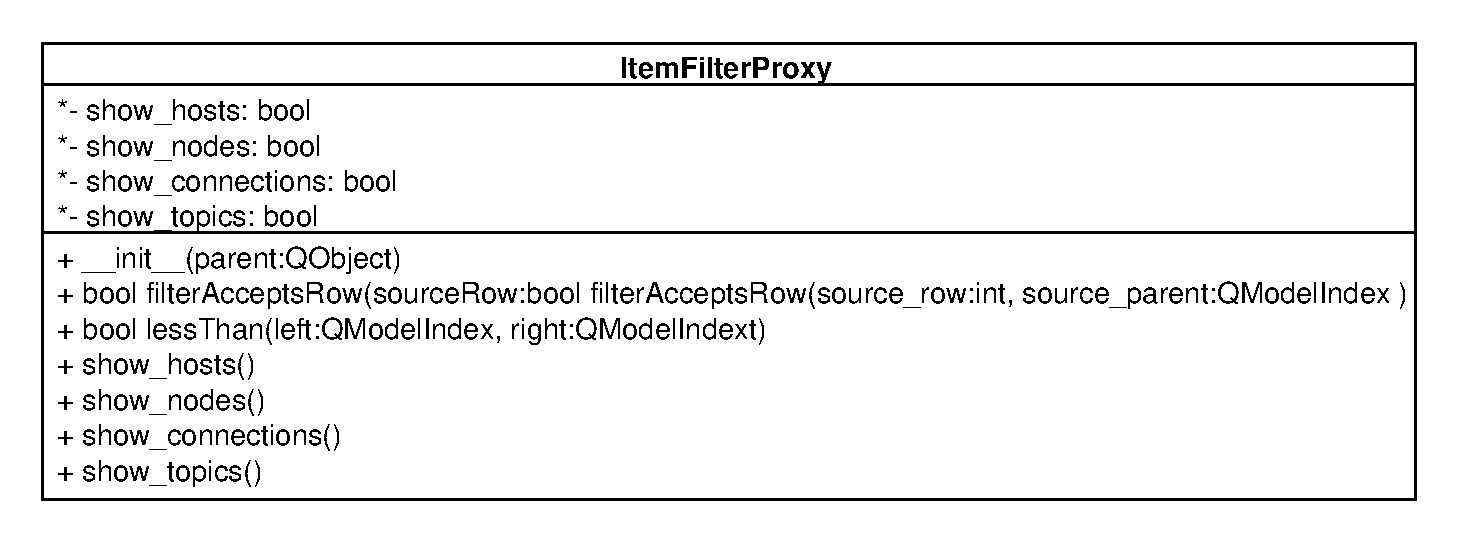
\includegraphics[scale=0.6]{./diagram_pictures/ItemFilter.pdf}
		\caption{The ItemFilterProxy}
	\end{minipage}
\end{figure} 
The ItemFilterProxy which is a QSortFilterProxyModel helps to filter the data going to the view so the user only sees what he wants to see (which he can modify by telling the view). 
\subsection{Attributes}
\begin{itemize}
  \item \textbf{private bool show\_hosts}\\
  True if hosts should be shown
  \item \textbf{private bool show\_nodes}\\
  True if nodes should be shown
  \item \textbf{private bool show\_connections}\\
  True if connections should be shown
  \item \textbf{private bool show\_topics}\\
  True if topics should be shown
\end{itemize}
\subsubsection{Methods}
\begin{itemize}
  %??
  %\item \textbf{public void \_\_init\_\_(QObject)}\\
  \item \textbf{public bool filterAcceptsRow(int source\_row, QModelIndex
  source\_parent)}\\
  Tells by analysing the given row if it should be shown or not. This behaviour can be modified via the show\_* methods or the setFilterRegExp method.
  \item \textbf{public bool lessThan(QModelIndex left, QModelIndex right)}\\
  Defines the sorting behaviour when comparing two entries of model item by telling how to compare these.
  \item \textbf{public void show\_hosts(bool show\_hosts)}\\
  Set true if hosts should be shown
  \item \textbf{public void show\_nodes(bool show\_nodes)}\\
  Set true if nodes should be shown
  \item \textbf{public void show\_connections(bool show\_connections)}\\
  Set true if connections should be shown
  \item \textbf{public void show\_topics(bool show\_topics)}\\
  Set true if topics should be shown
\end{itemize}

\subsection{LogFilterProxy}
\begin{figure}[htbp]
	\begin{minipage}[t]{7cm}
		\vspace{0pt}
		\centering
		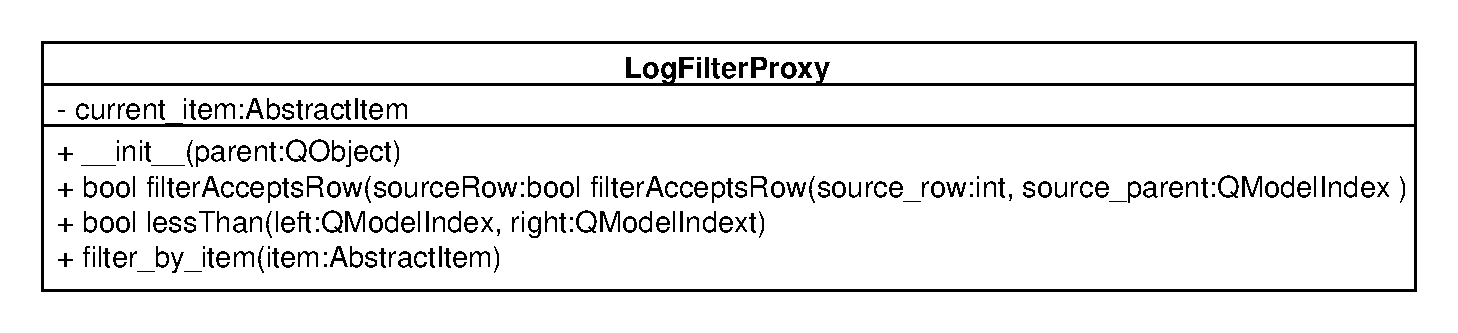
\includegraphics[scale=0.6]{./diagram_pictures/LogFilter.pdf}
		\caption{The LogFilterProxy}
	\end{minipage}	
\end{figure} 
The LogFilterProxy will especially be used to filter the complete log e.g. by a
specific node. This function is needed in the SelectionWidget where of course
only the log of the current selection should be shown.
\subsection{Attributes}
\begin{itemize}
  \item \textbf{private current\_item: AbstractItem}\\
  The currently selected item
\end{itemize}
\subsubsection{Methods}
\begin{itemize}
  %??
  %\item \textbf{public void \_\_init\_\_(QObject)}\\
  \item \textbf{public bool filterAcceptsRow(int source\_row, QModelIndex
  source\_parent)}\\
  Tells by analysing the given row if it should be shown or not. This behaviour can be modified via setFilterRegExp method so that e.g. only the entries of a specific host can be shown.
  \item \textbf{public bool lessThan(QModelIndex left, QModelIndex right)}\\
    Defines the sorting behaviour when comparing two entries of model item by telling how to compare these.
  \item \textbf{public void filter\_by\_item(AbstractItem item)}\\
  Used to tell the filter by which item it should filter. If the AbstractItem is None all log entries should be shown.
\end{itemize}

\subsection{SizeDelegate: QtGui.QStyledItemDelegate}
\begin{figure}[htbp]
	\begin{minipage}[t]{7cm}
		\vspace{0pt}
		\centering
		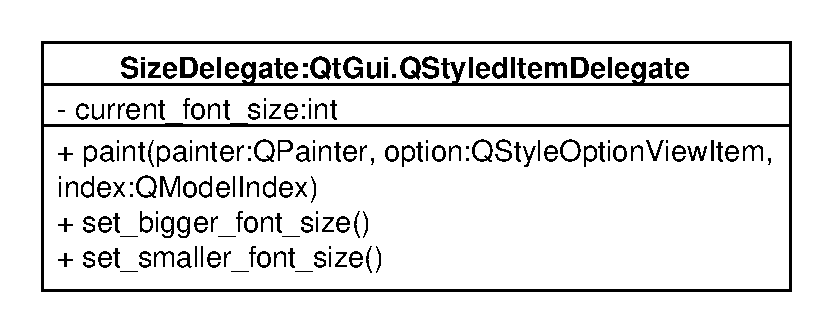
\includegraphics[scale=0.6]{./diagram_pictures/SizeDelegate.pdf}
		\caption{The ROSModel}
	\end{minipage}
	\hfill
	\begin{minipage}[t]{7cm}
		\vspace{10pt}
		Makes it possible to change the font size of the Gui-Plugin content
	\end{minipage}
\end{figure} 
\subsubsection{Attributes}
\begin{itemize}
  \item \textbf{private int current\_font\_size}\\
  The size displayed font
\end{itemize}
\subsubsection{Methods}
\begin{itemize}
  \item \textbf{public void paint(QPainter painter, QStyleOptionViewItem option,
  QModelIndex index)}\\
  Defines how the items of the model will be painted in the view. Can be used to draw e.g. bigger or smaller fonts.
  \item \textbf{public void set\_bigger\_font\_size()}\\
  Increases the displayed font-size
  \item \textbf{public void set\_smaller\_font\_size()}\\
  Decreases the displayed font-size
\end{itemize}

\newpage
\section{GUI - View}
\begin{figure}[!ht]
\begin{center}
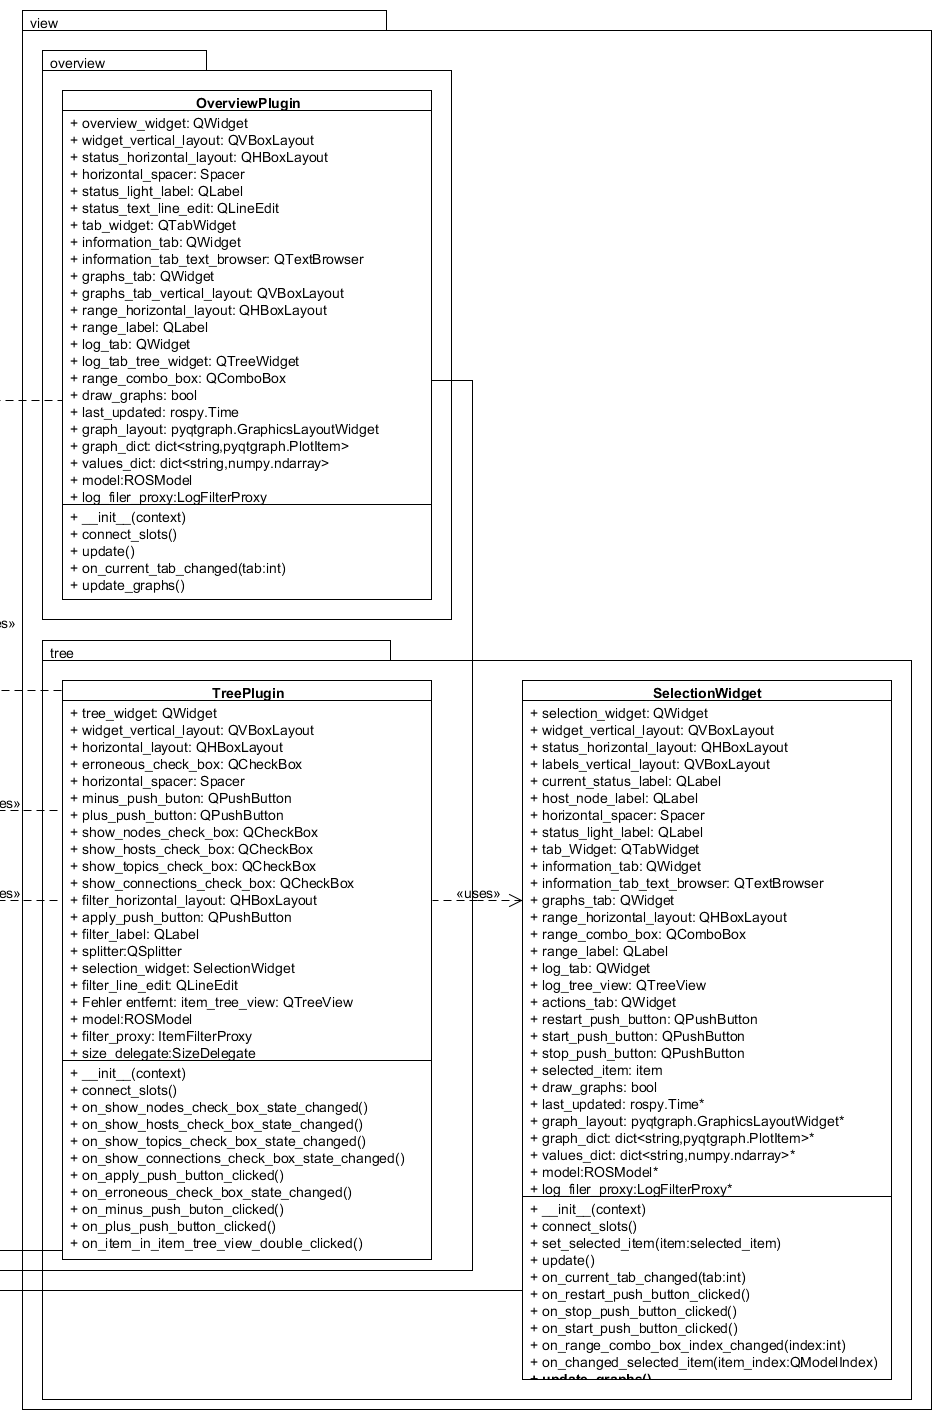
\includegraphics[width=0.8\linewidth]{./diagram_pictures/view.png}
\caption{The view class diagram}
\end{center}
\end{figure}

\subsection{OverviewPlugin}
\begin{figure}[htbp]
	\begin{minipage}[t]{7cm}
		\vspace{0pt}
		\centering
		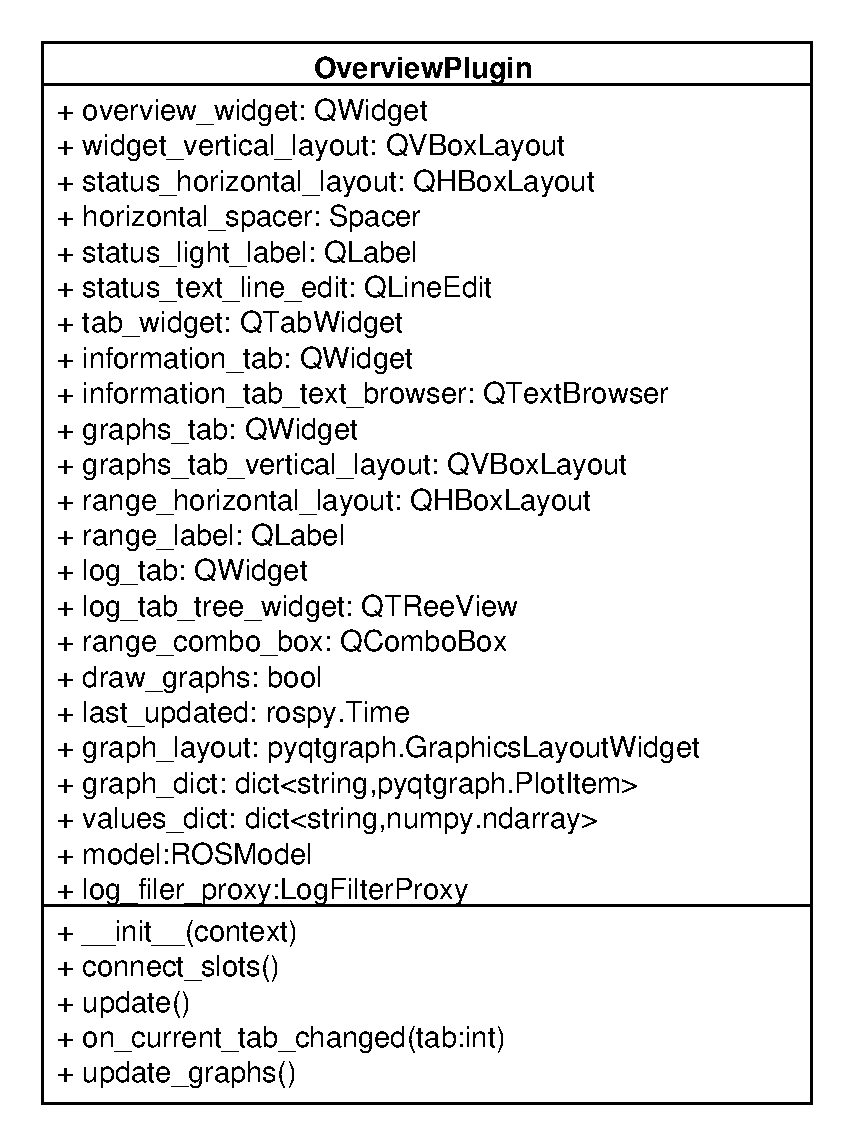
\includegraphics[scale=0.6]{./diagram_pictures/Overview.pdf}
		\caption{The ROSModel}
	\end{minipage}
	\hfill
	\begin{minipage}[t]{6.5cm}
		\vspace{10pt}
		The OverviewPlugin is the core of the graphical user interface, which
		contains most of the relevant information in a small and fancy area.
	\end{minipage}
\end{figure} 
\subsubsection{Attributes}
\begin{itemize}
  \item \textbf{public QWidget overview\_widget}\\
  The object which holds the widget
  \item \textbf{public QLabel status\_light\_label}\\
  A status ligth wich shows if everything is ok or not
  \item \textbf{public QTabWidget tab\_widget}\\
  The object wich holds the different tabs of the widget
  \item \textbf{public QWidget information\_tab}\\
  A tab wich gives general information about the network 
  \item \textbf{public QWidget graphs\_tab}\\
  Displays graphs about the network
  \item \textbf{public QComboBox range\_combo\_box}\\
  Makes it possible to set the range of the graphs
  \item \textbf{public QWidget log\_tab}\\
  Shows actual errors and warnings
  \item \textbf{public bool draw\_graphs}\\
  When the graph tab is selected, draw\_graphs is set on true an the graph will
  appear
  \item \textbf{public rospy.Time last\_update}\\
  The time of the latest update
  \item \textbf{public pyqtgraph.GraphicsLayoutWidget graph\_layout}\\
  The layout where the graphs will be plotted. Graphs are modelled as PlotItems.
  \item \textbf{public dict\{string, pyqtgraph.PlotItem\} graph\_dict}\\
  Dictionary of the names of the values together with the graphs represented as PlotItems.
  \item \textbf{public dict\{string, numpy.ndarray\} values\_dict}\\
  Dictionary of the names of the values together with the values as an array for fast plotting
  \item \textbf{public ROSModel model}\\
  The model used to show the content
  \item \textbf{public LogFilterProxy log\_fiter\_proxy}\\
  The LogFilterProxy which is currently used for sorting the logs.
  
\end{itemize}
\subsubsection{Methods}
\begin{itemize}
%   \item \textbf{public void \_\_init\_\_(context)}\\
%   ..
  \item \textbf{public void connect\_slots()}\\
  Initializes the slots of the widget
  \item \textbf{public void update()}\\
  Updates the widget and draws the graphs if draw\_graphs is true. 
  \item \textbf{public void on\_current\_tab\_changed(int tab)}\\
  The widget wants to get notified when the tab changed so it can e.g. draw the graphs etc.
  \item \textbf{public void update\_graphs()}\\
  Updates and redraws the graphs
\end{itemize}

\newpage
\subsection{TreePlugin}
\begin{figure}[htbp]
	\begin{minipage}[t]{7cm}
		\vspace{0pt}
		\centering
		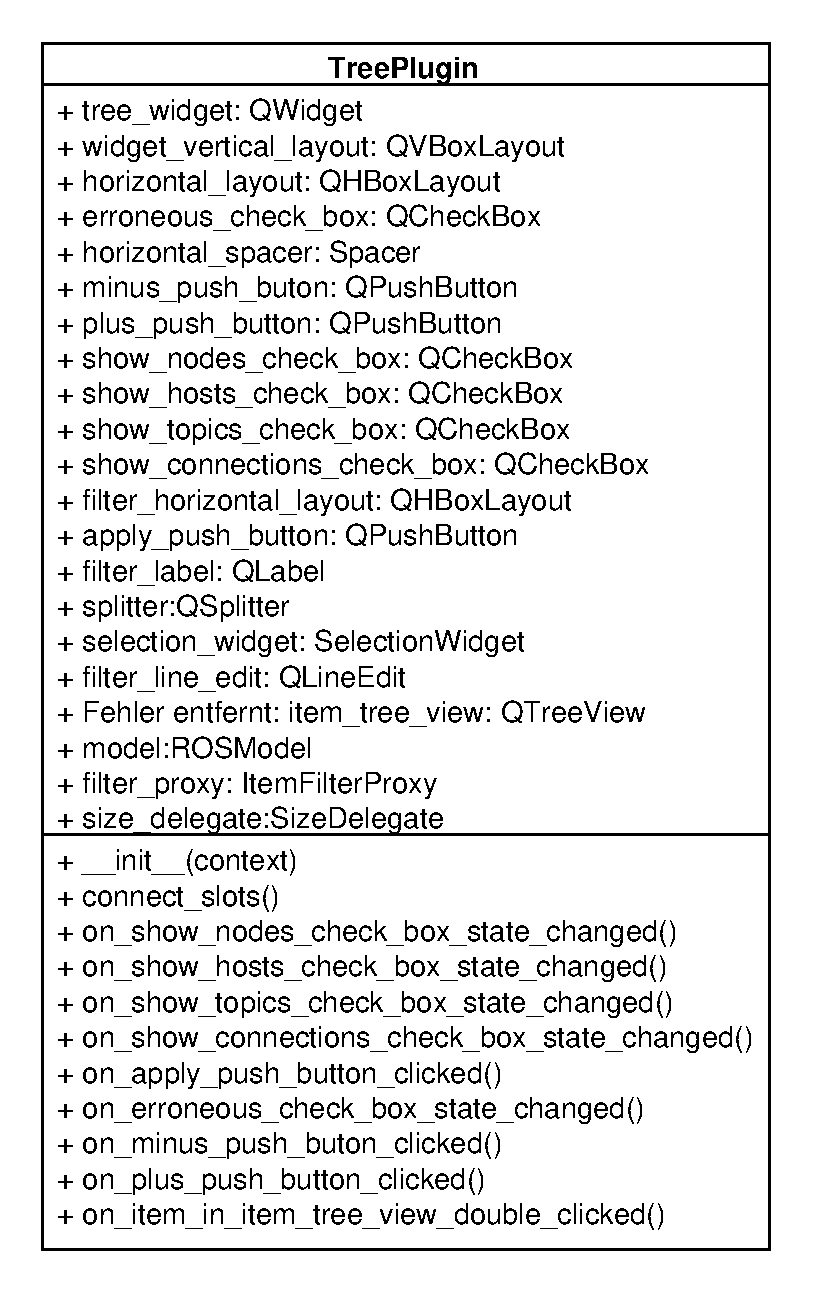
\includegraphics[scale=0.6]{./diagram_pictures/Tree.pdf}
		\caption{The ROSModel}
	\end{minipage}
	\hfill
	\begin{minipage}[t]{5.5cm}
		\vspace{10pt}
		TreePlugin is very simply and shows only the actual active hosts
		and nodes. It is possible to filter the output, e.g. only erroneus hosts or
		nodes are displayed.
	\end{minipage}
\end{figure} 
\subsubsection{Attributes}
\begin{itemize}
  \item \textbf{public QWidget tree\_widget}\\
  The object wich holds the widget
  \item \textbf{public QCheckBox erroneous\_check\_box}\\
  Only erroneous hosts and nodes will be displayed
  \item \textbf{public QCheckBox show\_node\_check\_box}\\
  Displays the activ nodes
  \item \textbf{public QCheckBox show\_host\_check\_box}\\
  Displays the activ hosts
  \item \textbf{public QCheckBox show\_topics\_check\_box}\\
  Displays the actual topics
  \item \textbf{pubic QCheckBox show\_connects\_check\_box}\\
  Displays the actual connections
  \item \textbf{public QPushButton plus\_push\_button}\\
  Makes it for, a better clarity, possible to zoom in  
  \item \textbf{public QPushButton minus\_push\_button}\\
  and zoom out
  \item \textbf{public SelectionWidget selection\_widget}\\
  The SelectionWidget which opens on double-click on the TreeView
  \item \textbf{public QLineEdit filter\_line\_edit}\\
  A textfield where you can define a filter for the output
  \item \textbf{public ROSModel model}\\
  The connection to the ROSModel
  \item \textbf{public ItemFilterProxy filter\_proxy}\\
  The filter which will be used to filter the items of the TreeViews e.g. by a search text or according to other criteria selectable by CheckBoxes like show\_hosts.
  \item \textbf{private size\_delegate: SizeDelegte}\\
  The size\_delegate is responsible for painting the rows in a specific manner e.g. to make the font bigger.
  
\end{itemize}
\subsubsection{Methods}
\begin{itemize}
%   \item \textbf{public void \_\_init\_\_(context)}\\
%   ..
  \item \textbf{public void connect\_slots()}\\
  Initializes the slots from the widget
  \item \textbf{public void on\_show\_nodes\_check\_box\_state\_changed(bool activated)}\\
  Displays or delete the nodes in the box wether the check box is set or unset
  \item \textbf{public void on\_show\_hosts\_check\_box\_state\_changed(bool activated)}\\
  Displays or delete the host in the box wether the check box is set or unset
  \item \textbf{public void on\_show\_topics\_check\_box\_state\_changed(bool activated)}\\
  Displays or delete the topics in the box wether the check box is set or unset
  \item \textbf{public void
  on\_show\_connections\_check\_box\_state\_changed(bool activated)}\\
  Displays or delete the connections in the box wether the check box is set or
  unset
  \item \textbf{public void on\_apply\_push\_button\_clicked()}\\
  Filters the content in the box according to the content of the
  filter\_line\_edit
  \item \textbf{public void on\_erroneus\_check\_box\_state\_changed()}\\
  If this check box is set, only erroneus hosts and nodes will be displayed  
  \item \textbf{public void on\_plus\_push\_button\_clicked()}\\
  Checks if the plus\_push\_button is clicked and zoomes in (increases the size
  of the font)
  \item \textbf{public void on\_minus\_push\_button\_clicked()}\\
  Checks if the minus\_push\_button is clicked and zoomes out (decreases the
  size of the font)
  \item \textbf{public void on\_item\_in\_tree\_view\_double\_clicked()}\\
  Handels the double-click action and opens the clicked item in the SelectionWidget
\end{itemize}

\newpage
\subsection{SelectionWidget}
\begin{figure}[htbp]
	\begin{minipage}[t]{7cm}
		\vspace{0pt}
		\centering
		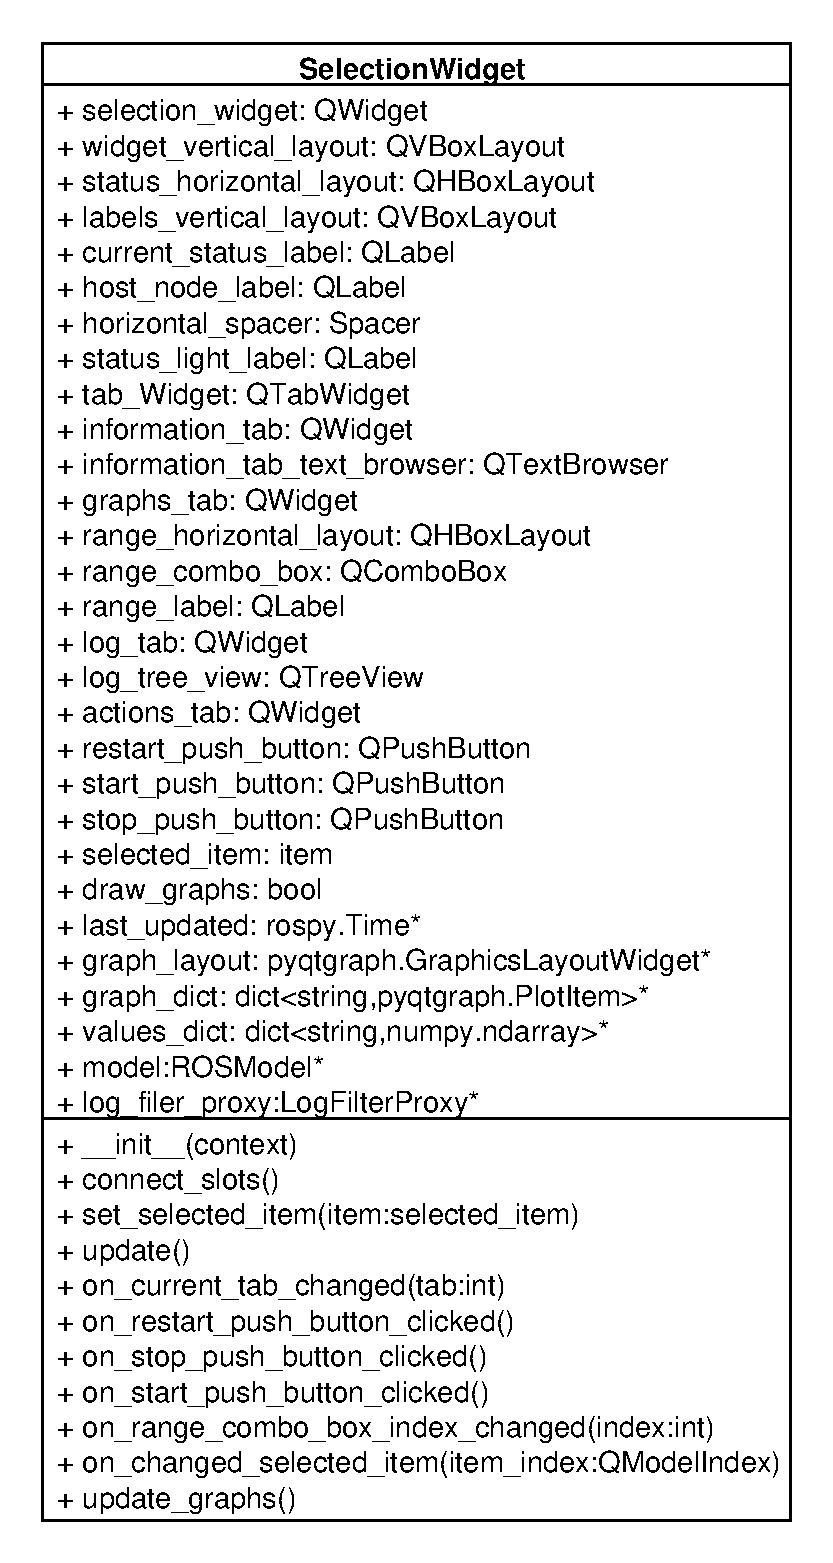
\includegraphics[scale=0.6]{./diagram_pictures/Selection.pdf}
		\caption{The ROSModel}
	\end{minipage}
	\hfill
	\begin{minipage}[t]{6.5cm}
		\vspace{10pt}
		This Widget shows detailed information the currently selected item which might be a host, a node, a topic or a connection.
	\end{minipage}
\end{figure} 
\subsubsection{Attributes}
\begin{itemize}
  \item \textbf{public QLabel host\_node\_label}\\
  The name of the actual selected item
  \item \textbf{public QLabel status\_light\_label}\\
  A status-light about the status of the current item
  \item \textbf{public QTabWidget tab\_widget}\\
  The object wich holds the different tabs of the widget
  \item \textbf{public QWidget information\_tab}\\
  A tab wich gives general information about hosts or nodes 
  \item \textbf{public QWidget graphs\_tab}\\
  Displays graphs about the actual selected item, e.g the Network- and
  CPU-Load
  \item \textbf{public QComboBox range\_combo\_box}\\
  Makes it possible to set the range of the graphs
  \item \textbf{public QWidget log\_tab}\\
  Shows actual errors and warnings
  \item \textbf{public QWidget actions\_tab}\\
  Includes buttons to restart and stop nodes
  \item \textbf{public item selected\_item}\\
  The selected item
  \item \textbf{public bool draw\_graphs}\\
  When the graph tab is selected, draw\_graphs is set on true an the graph will
  appear
  \item \textbf{public rospy.Time last\_updated}\\
  The time of the last update
  \item \textbf{public dict\{string, pyqtgraph.PlotItem\} graph\_dict}\\
  Dict of the names of the values together with the graphs represented as PlotItems.
  \item \textbf{public dict\{string, numpy.ndarray\} values\_dict}\\
  Dictionary of the names of the values together with the values as an array for fast plotting
  \item \textbf{public ROSModel model}\\
  The model used to show the content
  \item \textbf{public LogFilterProxy log\_filter\_proxy}\\
  The filterproxy which will be used to show only the entries of the current item in the log\_tab
  
\end{itemize}
\subsubsection{Methods}
\begin{itemize}
%   \item \textbf{public void \_\_init\_\_(context)}\\
%   ..
  \item \textbf{public void connect\_slots()}\\
  Initializes the slots from the widget
  \item \textbf{public void set\_selected\_item(item selected\_item)}\\
  Set the selected item
  \item \textbf{public void update()}\\
  Updates the widget
  \item \textbf{public void on\_current\_tab\_changed(int tab)}\\
  Will be called when you switch between tabs
  \item \textbf{public void on\_restart\_push\_button\_clicked()}\\
  Handels the retart button and restarts a host or node
  \item \textbf{public void on\_stop\_push\_button\_clicked()}\\
  Handels the stop button and stops a host or node
  \item \textbf{public void on\_start\_push\_button\_clicked()}\\
  Handels the start button and starts ahost or node
  \item \textbf{public void on\_range\_combo\_box\_index\_changed(int index)}\\
  Handels the change of the graph range
  \item \textbf{public void on\_changed\_selected\_item(QModelIndex)}\
  Item\_index\ handels the change of the selected item
  \item \textbf{public void update\_graphs()}\\
  Updates the graph plot
\end{itemize}